\section{Wrapper}\label{sec:Wrapper}
%OSS: Explain that the wrapper was originally conceived of as a role, is it now? Does it need to be renamed?
\subsubsection*{Motivation} This pattern suggests to find at least one person to fill an important role managing the project's public interface, and keeping participants up to date about activities.

%% \begin{center}
%% \begin{tabular}{l}
%% \textbf{$\leftarrow$\patternname{Roadmap}: If project participants are not all contributing, someone may take charge of the plan.}\\
%% \textbf{$\leftarrow$\patternname{Scrapbook}: Someone may also need to take change of gathering outstanding concerns.}\\
%% \end{tabular}
%% \end{center}

\subsubsection*{Context} You are part of an active, long-running, and possibly quite complex project with more than a handful of participants.  How do you manage?

\subsubsection*{Forces}~
\begin{tabular}[t]{p{.8\textwidth}@{\hspace{.03\textwidth}}c}
\textbf{Interface}: the project shows people how they can use it. & {\icon \symbol{"002136}} \\
\textbf{Familiarity}: the leader/follower dichotomy is easy to understand. &  {\icon \symbol{"0021B2}} \\
\textbf{Equity}: peeragogy aims for fairness. &  {\icon \symbol{"0021BD}} \\
\end{tabular}

\subsubsection*{Problem} In an active project, it can be effectively impossible to stay up to date with all of the details.  Not everyone will be able to attend every meeting (see \patternname{Heartbeat}) or read every email.  Project participants can easily get lost and drift away.  The experience can be much more difficult for \patternnameplural{Newcomer}: joining an existing project can feel like trying to climb aboard a rapidly moving vehicle.  If you've taken time off, you may feel like things have moved on so far that you cannot catch up.  Information overload is not the only concern: there is also a problem with missing information.  If key skills are not shared, they can quickly become bottlenecks (see \patternname{Carrying capacity}).

\subsubsection*{Solution}
% DK: Be more direct.  Don’t say what “can” be done…just say what to do. [also, typo -jc]
Someone involved with the project should regularly create a wrap-up
summary, distinct from other project communications, that makes
current activities comprehensible to people who may not have been
following all of the details.  In addition, project members should
keep other informative resources like the landing page,
\patternname{Roadmap}, and documentation up to date.  Check
empirically to see if they really show interested parties how they can
get involved.  Building on the idea of a ``project
dashboard'' in Figure \ref{dashboard}, we can guide potential
contributors to live help; we can then see what questions they
ask.\footnote{\url{https://gitter.im/orgs/Peeragogy/rooms}}  The
\patternname{Wrapper} is both a role, and, sometimes, an artifact.
Our \emph{Handbook}'s cover literally wraps up its contents; the
collaboratively written chat notes from our weekly Hangouts give a
collaboratively-written overview of what was discussed in the meeting.
Meetings themselves can be structured to give people a chance to sum
up what they've accomplished during the week, as well as any problems
they are running into.  Between meetings, each participant is advised
to maintain some sort of ``learning log'' in the form of a personal
\patternname{Scrapbook}, so that outstanding concerns are surfaced and
available to discuss.

\subsubsection*{Rationale}
According to the theory proposed by Yochai Benkler, for free/open ``commons-based'' projects to work, it is important for participants to be able to contribute small pieces, and for the project to have a way to stitch those pieces together \cite{coases-penguin}. The \patternname{Wrapper} helps perform this integrative stitching function. If you value participation, you may have to do some serious work to facilitate access to process.

\subsubsection*{Resolution} 
% DK: This sounds like Rationale
Well-maintained records chronicle the project's history; up-to-date documentation makes the project more robust; a coherent look-and-feel offers an accessible \textbf{interface} to the outside world. Regularly circulated summaries can help to engage or re-engage members of a project, and can give an emotional boost to peeragogues who see their contributions and concerns mentioned, giving less engaged participants the \textbf{familiar} experience of ``following'' someone else's updates. People will judge from experience whether the project strives for \textbf{equity} or strives to maintain hidden power differentials.  

\subsubsection*{Example 1} 
There are many data streams around the Wikimedia project.  They comprise an elaborate \patternname{Wrapper} function for the project, with components that range from Today's Featured Article, which appears on the front page of Wikipedia, to formal annual reports from the nonprofit.\footnote{\url{https://en.wikipedia.org/wiki/Wikipedia:Today\%27s_featured_article}}\textsuperscript{,}\footnote{\url{https://wikimediafoundation.org/wiki/Annual_Report}}

%% That said, citing Wikipedia in academic writing remains controversial.
%% One team of researchers found that, all else equal, when a scientific article is
%% cited on Wikipedia, that does not make it more likely to be cited
%% elsewhere \cite{marashi2013impact}.  These facts suggest that Wikipedia 
%% provides a relatively ``thin'' and non-distorting window on the world.

\subsubsection*{Example 2} In-person meetings are just as relevant for contemporary humans as they were a century ago, even though we often work remotely, and have learned more about how to assemble on the fly \cite{rheingold2007smart}.  Getting together for conventions, dance parties, and commencement ceremonies could comprise an important part of the future university's \patternname{Wrapper} function, even if these events do not always take place in one specific Assembly Hall.

%\subsubsection*{Summary}

\begin{figure}[t]
{\centering
\resizebox{.85\textwidth}{!}{
\begin{tikzpicture}[every node/.style={anchor=south west,inner sep=0pt},x=1mm, y=1mm,]
     \node (fig1) at (0,0)
       {\includegraphics[width=\textwidth,trim=0mm 135mm 0mm 0mm,clip=true]{figures/peeragogy_dashboard_draft1/peeragogy_dashboard_draft1.jpg}};
     \node (fig2) at (54, 15)
       {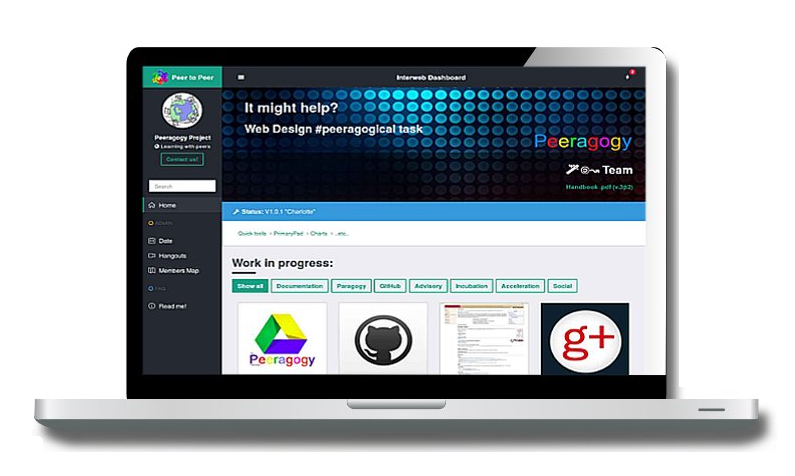
\includegraphics[width=.45\textwidth,trim=10mm 10mm 10mm 10mm,clip=true]{figures/dashboard/dash-trans.png}};  
\end{tikzpicture}
}

\par}
\caption{Design for a Peeragogy project dashboard (sketch by Amanda Lyons, prototype by Fabrizio Terzi; images used with permission).\label{dashboard}}
\end{figure}

\FloatBarrier

\begin{framed}
\noindent 
\emph{What's Next in the Peeragogy Project}
\definecollection{WrapperWN}
\begin{collectinmacro}{\WrapperWN}{}{}
Let's make sure we have protocols in place that enable us to share
progress, and to revise our ``next steps'' if people are getting
stuck.  Let's improve the interaction design for peeragogy.org so that
it's clear how people can get involved.
\end{collectinmacro}
\WrapperWN
\end{framed}    

%\newpage
